% !TEX encoding = UTF-8
% !TEX TS-program = pdflatex
% !TEX root = ../tesi.tex

%**************************************************************
\chapter{Descrizione dello stage}
\label{cap:descrizione-stage}
%**************************************************************

\intro{Breve introduzione al capitolo}\\

In questo capitolo viene descritto come si è pianificato e svolto lo stage presso SAI, introducendo il progetto, considerando gli obiettivi e i possibili rischi.

%**************************************************************
\section{Introduzione al progetto}

o stage svolto presso SAI aveva come scopo la creazione di un prototipo di piattaforma web/desktop per il caricamento delle registrazioni audio effettuate nelle aule di tribunale, con l'aiuto di alcuni metadata prodotti durante le medesime registrazioni. In particolare l'applicazione da sviluppare è divisa in due parti backend e frontend (spiegare meglio back e front) che comunicano tra loro mediante API rest (spiegare API). Lo stage si è focalizzato sullo sviluppo della parte frontend, avanzando di pari passo con lo sviluppo del  backend realizzata da altri membri del team di sviluppo. Per la realizzazione del frontend si è scelto di utilizzare Javascript con i framework React e Redux.

%**************************************************************
\section{Analisi preventiva dei rischi}

Nella fase di analisi iniziali si sono individuati i principali rischi a cui si poteva andare incontro e si è proceduto a definire le possibili soluzione per farne fronte.\\

\begin{risk}{Uso di nuove tecnologie}
  \riskdescription{le tecnologie proposte per la gestione e lo sviluppo del progetto erano per lo più nuove o scarsamente conosciute.}
  \risksolution{è stato previsto un periodo iniziale di studio e formazione su queste tecnologie.}
  \label{risk:new-tecnology}
\end{risk}
\begin{risk}{Modalità di lavoro smart working}
  \riskdescription{lo stage è stato fatto completamente da remoto, e poteva portare ad una possibile mancanza di comunicazione e ad un incertezza nelle attività da svolgere.}
  \risksolution{il tutor aziendale si è reso disponibile a vari meeting nelle prime fasi del progetto e nella formazione iniziale, e rimanendo a disposizione per altri meeting  in caso di dubbi sulle attività da svolgere.}
  \label{risk:smart-working}
\end{risk}

%**************************************************************
\section{Requisiti e obiettivi}

Si farà riferimento ai requisiti secondo le seguenti notazioni:
\begin{itemize}
  \item O per i requisiti obbligatori, vincolanti in quanto obiettivo primario richiesto dal committente;
  \item D per i requisiti desiderabili, non vincolanti o strettamente necessari, ma dal riconoscibile valore aggiunto;
  \item F per i requisiti facoltativi, rappresentanti valore aggiunto non strettamente competitivo.
        Le sigle precedentemente indicate saranno seguite da una coppia sequenziale di numeri, identificativo del requisito.
\end{itemize}

\begin{table}
  \caption{Your caption}
  \label{tab:table}
  \centering
  \begin{tabularx}{\linewidth}{|>{\hsize=.8\hsize}X|>{\hsize=1.2\hsize}X|}
    \toprule
    \hline
    O01 & autenticazione mediante server remoto                                               \\
    \hline
    O02 & lettura dati da CD                                                                  \\
    \hline
    O03 & precompilazione di form con i dati caricati da CD                                   \\
    \hline
    O04 & editing dei dati del form                                                           \\
    \hline
    D01 & upload dei dati verso i sistemi esterni                                             \\
    \hline
    D02 & test di unità esaustivi                                                             \\
    \hline
    F01 & possibilità di ascoltare le registrazioni                                           \\
    \hline
    F02 & possibilità di modificare i dati mediante interazioni evolute (per es. drag-n-drop) \\
    \hline
    F03 & realizzazione di un’applicazione desktop con Electron                               \\
    \hline
    F04 & compilazione multipiattaforma dell’applicazione desktop                             \\
    \hline
  \end{tabularx}
\end{table}

%**************************************************************
\section{Pianificazione}

La pianificazione, in termini di quantità di ore, sarà distribuita in attività di studio e attività implementative.

Lo stage è stato strutturato in due fasi principali, la prima dedicata alle attività di studio e la seconda alle attività implementative. Di seguito vengono elencate le attività pianificate con la relativa quantità di ore stimata per ogni attività.

\begin{itemize}
  \item Studio delle tecnologie (80 ore)
        \begin{itemize}
          \item Setup di un prototipo di applicazione React e del backend (16 ore);
          \item Studio delle librerie necessarie (React, Redux, JWT, OAuth) (64 ore);
        \end{itemize}
  \item Implementazione prototipo (240 ore)
        \begin{itemize}
          \item Realizzazione dell’interfaccia di login (30 ore);
          \item Implementazione lettura e visualizzazione dei dati da CD (70 ore);
          \item Implementazione editing dei dati letti da CD (70 ore);
          \item Implementazione upload dei dati (30 ore);
          \item Testing dei prodotti realizzati (40ore);
        \end{itemize}
\end{itemize}

Per ogni attività riguardante la fase di implementazione del prototipo è stata prevista anche la relativa attività di testing.
Il tutto viene rappresentato dal seguente dal diagramma di Gantt.
\begin{center}
  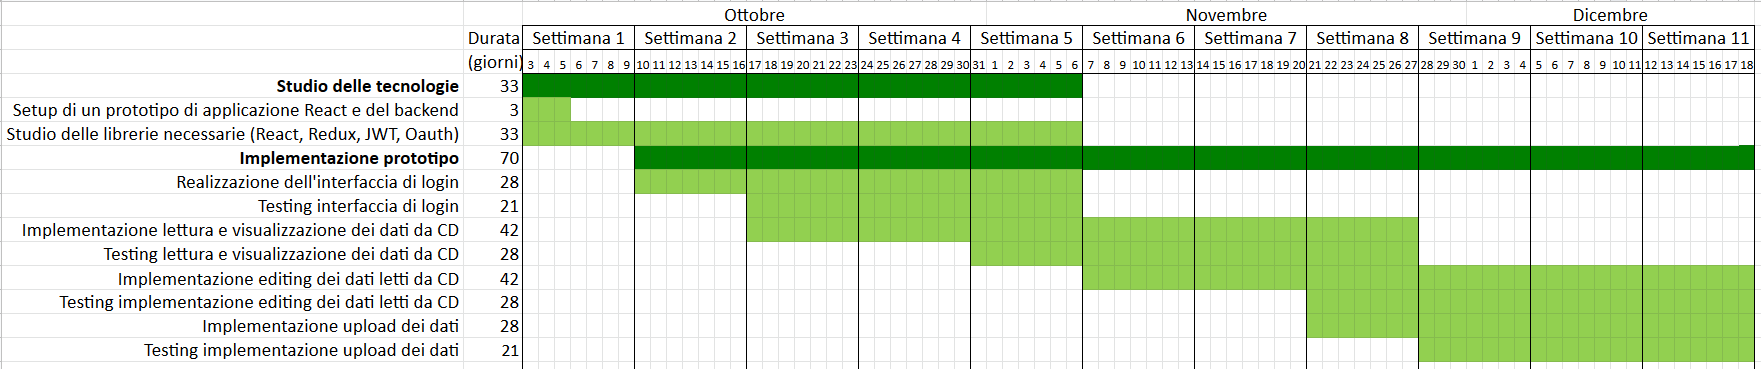
\includegraphics[width=14cm]{gantt}
\end{center}